\chapter{Business Model} % (fold)
\label{cha:business_model}


\section{Markt Potential and Customer Segments} % (fold)
\label{sec:markt_potential_and_customer_segments}
Most of Legacy’s customers are expected to fit one of the following categories:
\begin{itemize}
	\item People in their mid-thirties, who are moving in with a significant other or having kids. They are experiencing the first memories of building their own family, and want to preserve them.
	\item Baby Boomers and seniors: people who start planning the last stage of their lives and/or those suffering illness. They feel at the end of their journey, and want to share what they learned and experienced.
	\item Professionals in a high-risk environment, such as firefighters, loggers, fishermen, etc.
	\item People needing a proven “dead man switch” to distribute documents.
\end{itemize}

Legacy is oriented to the average internet user. We put special focus on seniors  and baby boomers, as this public might feel particularly concerned with the problems that Legacy aims to solve. As a result, the Legacy interface is designed in order to be simple and intuitive. In principle, since both Memoirs and Heritage releases should not involve major legal issues, access to the global market is envisaged. Future releases including enhanced capabilities (i.e., cryptocurrencies, smart property) throughout different countries will require a case-to-case study regarding the specificities of each local regulation and will be deployed progressively. Particular attention (in terms of language, legal and customer support) will be given to markets where the demand for next-generation digital services is potentially higher, i.e., the European, Asian and North American markets. Business expansion to other regions is foreseen at a later stage, according to the observed demand.  

The rapid growth of the overall cryptocurrency market capitalisation has also given rise to another significant market segment. As mentioned above, holders of cryptocurrency currently lack of a reliable mechanism to secure their holdings in case of decease. Legacy is the first platform aiming at tackling this issue. Similarly, smart property will require reliable transfer and distribution mechanisms, which brings additional market opportunities. 

% section markt_potential_and_customer_segments (end)

\section{Competitive Analysis and Unfair Advantage} % (fold)
\label{sec:competitive_analysis_and_unfair_advantage}

Several competitors claim to offer a product similar to Legacy (see for instance \url{legacyvault.com} and \url{knotify.me}). Most of these services, however, are based on a centralized structure, making their customers vulnerable to a single point of failure: the company hosting the service. Some cited examples in the appendix show some that have already closed at the time of writing this document.

Most of the competitors also rely on an annual billing cycle, making the service total price an unknown quantity. By contrast, Legacy offers a one-time payment option, offering the peace of mind that memories will not be lost should the customer suffer hardship in his future.

Two examples that are exceptions in our competition analysis are lastwill.io and digipulse.io, both of which, to some extent, are blockchain based services. But both have a limited view of what the smart will can do, and mainly target cryptocurrency owners, which we believe is a mistake in the market analysis.

The durable, auditable, and transparent nature of Legacy, detailed below, places it in a category of its own.


\section{Service Operation, Fees and Revenue} % (fold)
\label{sec:service_operation_fees_and_revenue}
Legacy users are able to sign-up to the application for free. A free account allows to explore the application interface, upload files (memories) and organize them into capsules. A subscription is required in order to commit a capsule. From a technical point of view, committing a capsule results in the creation of a smart contract on the blockchain and the initiation of the PoL engine, which involves transaction and operational fees. Subscripted users also benefit from a secure, decentralized file storage system.

Several subscription packages will be proposed. These differ according to the amount of storage capacity, PoL reliability level and additional services such as special customer support, including legal advice or access to professional storytelling specialists.

Subscription fees will be charged on a lifetime or periodic basis, and can be paid through fiat currencies as well as through conventional cryptocurrencies such as ether. In addition, subscription fees may be paid through the Legacy token, which provides users with commercial advantages.

The target price of the lifetime Legacy subscription is between 250€ and 500€.
% section service_operation_fees_and_revenue (end)

\section{Customer Relations and Channels} % (fold)
\label{sec:customer_relations_and_channels}
Convincing user to entrust their memories to Legacy implies building long-term confidence in our product.
For all segments, marketing campaigns will be carried mainly on the web in order to bring potential customers to the website where they can sign-up.
Legacy will also partner with players in specific markets, such as life insurance providers. The Legacy service can be bundled in global offers, in particular from established players in the Silver Economy.
The most costly part of the customer relationship will be providing tailored legal advice to specific customers: this will be part of a premium package.

In all cases, Legacy will provide powerful onboarding tools to make the experience as simple as possible, such as automatically building capsules and contacts based on social network activity.
% section customer_relations_and_channels (end)

\section{Cost Structure} % (fold)
\label{sec:cost_structure}
Most of Legacy’s costs will come from the team salaries. For details, see Section \ref{Resource Allocation}.
Each customer will also have a recurring cost for Proof of Life verification. We estimate the average customer to be around 48 years old. Taking into account a life expectancy of 80 years, the average service duration for a customer is calculated at 32 years.

Using the estimates outlined in this section, Legacy will become profitable in 2022, with 8 million USD needed in funding to reach that goal.

\begin{figure}[h]
  \centering
  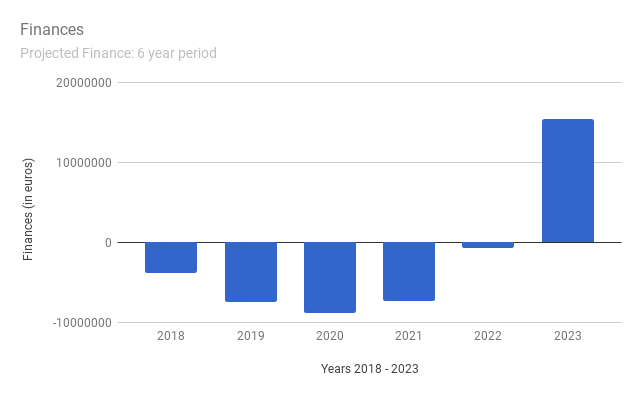
\includegraphics[scale=0.5]{fig/finances_chart}
  \caption{Projected finances: 6-year time span.}
  \label{fig:ACRDA_SIC}
\end{figure} 

% section cost_structure (end)

% chapter business_model (end)